\documentclass[conference]{IEEEtran}
\IEEEoverridecommandlockouts
\usepackage{cite}
\usepackage{amsmath,amssymb,amsfonts}
\usepackage{algorithmic}
\usepackage{graphicx}
\usepackage{textcomp}
\usepackage{xcolor}
\usepackage{array}

% ---------------------------------------------------------------------------
% Float placement.
%
% placeins/\FloatBarrier was removed deliberately. A barrier forces every
% pending float to be *placed* before the following text may start, so when the
% next float does not fit in the remaining column, LaTeX ends the column early
% and leaves the rest of the page blank. That was the direct cause of the large
% gaps.
%
% Instead: loosen the fractions so floats may settle at the top OR bottom of a
% column near the text that references them. \bottomfraction defaults to 0.3,
% which silently rejects almost every figure here as a bottom float; raising it
% is what lets the half-column-height figures fill the space they were leaving
% empty.
% ---------------------------------------------------------------------------
\renewcommand{\topfraction}{0.9}
\renewcommand{\bottomfraction}{0.7}
\renewcommand{\textfraction}{0.07}
\renewcommand{\floatpagefraction}{0.75}
\renewcommand{\dblfloatpagefraction}{0.75}
\renewcommand{\dbltopfraction}{0.9}
\setcounter{topnumber}{4}
\setcounter{bottomnumber}{2}
\setcounter{dbltopnumber}{4}
\setcounter{totalnumber}{6}

\def\BibTeX{{\rm B\kern-.05em{\sc i\kern-.025em b}\kern-.08em
    T\kern-.1667em\lower.7ex\hbox{E}\kern-.125emX}}
\begin{document}

\title{Z-Shift: A Unified Ingestion-to-Deliverable Pipeline for 
Converting Heterogeneous 2D Media into Refined 3D Assets}

% Author block is laid out 3 + 3. The \linebreak after the third author forces
% the second row; without it IEEEtran fits only two blocks per row, because the
% department line is wide. The department is split over two lines for the same
% reason -- if you restore it to a single line, three blocks will not fit.
\author{\IEEEauthorblockN{Sidhant Kishore}
\IEEEauthorblockA{\textit{School of Computer Science} \\
\textit{and Engineering} \\
\textit{Vellore Institute of Technology}\\
Vellore, India \\
email@vitstudent.ac.in}
\and
\IEEEauthorblockN{Rakshit Mathur}
\IEEEauthorblockA{\textit{School of Computer Science} \\
\textit{and Engineering} \\
\textit{Vellore Institute of Technology}\\
Vellore, India \\
rakshitmathur2025@vitstudent.ac.in}
\and
\IEEEauthorblockN{Jhanvi Vashishth}
\IEEEauthorblockA{\textit{School of Computer Science} \\
\textit{and Engineering} \\
\textit{Vellore Institute of Technology}\\
Vellore, India \\
email@vitstudent.ac.in}
\and
\IEEEauthorblockN{Shardul Parag}
\IEEEauthorblockA{\textit{School of Computer Science} \\
\textit{and Engineering} \\
\textit{Vellore Institute of Technology}\\
Vellore, India \\
email@vitstudent.ac.in}
\and
\IEEEauthorblockN{Ayush Kumar}
\IEEEauthorblockA{\textit{School of Computer Science} \\
\textit{and Engineering} \\
\textit{Vellore Institute of Technology}\\
Vellore, India \\
theofficialayush.kumar@gmail.com}
\and
\IEEEauthorblockN{Given Name Surname}
\IEEEauthorblockA{\textit{School of Computer Science} \\
\textit{and Engineering} \\
\textit{Vellore Institute of Technology}\\
Vellore, India \\
email@vitstudent.ac.in}
}

\maketitle

% Pulls the abstract up under the 3+3 author block. IEEEtran leaves a fixed
% gap below \author, sized for a one- or two-row block of short affiliations;
% with six four-line blocks it reads as a hole. -14pt closes it without
% crowding the rule above the abstract. If the author list ever shrinks to one
% row, drop this -- the default spacing is correct at that size.
\vspace{-14pt}

\begin{abstract}
DUSt3R and MASt3R recover dense geometry from a scene based on 2D observations
alone, without requiring information about camera pose and without prior
calibration. A readily deployable 2D-to-3D system, however, cannot be built
from the reconstruction network by itself: ingestion, frame selection,
temporal synchronization, geometry refinement, and application-specific
delivery must operate in concert. We present z-shift, a four-stage pipeline in
which each individual stage can be replaced if desired, and in which data
passes between stages only as serializable artifacts. During ingestion,
images, videos, synchronized captures, and live feeds are unified into a
common spatial schema. Reconstruction uses MASt3R for its initial estimate of
scene geometry, may optionally fuse TSDFs, and falls back to a point map where
fusion is unavailable. Refinement applies a fixed sequence of operations, and
delivery routes GLB or point-cloud output under a compatibility contract. Our
evaluation consists of a constrained benchmark suite together with one eight-
view capture in which each stage was individually traced. Unless capture order
is preserved, motion-ranked frame retention degrades sliding-window pairing
locality by 6.6x, and restoring that order costs nothing. Refinement cost is
affected by the number of disconnected components in a mesh more than by its
triangle count, remaining nearly constant below approximately 100 components
and rising close to linearly thereafter, reaching 23x at 1,000. Repeating a
run on the same GPU under the same configuration produces byte-identical
output. Component- and integration-level correctness is established across the
pipeline. Real-time delivery, efficient large-scale mesh processing, and
quantitative reconstruction accuracy against ground truth remain future work.
\end{abstract}

\begin{IEEEkeywords}
3D reconstruction, multi-view stereo, MASt3R, computer vision, mesh processing,
point clouds, 2D-to-3D generation, spatial computing
\end{IEEEkeywords}

\section{Introduction}

Computer vision and graphics have long treated the recovery of three-dimensional
structure from two-dimensional images as a foundational problem. From multiple
observations, classical structure-from-motion (SfM) and multi-view stereo (MVS)
methods estimate camera geometry, correspondences, depth, and surfaces
\cite{b1}--\cite{b4}; their accuracy nonetheless depends on viewpoint coverage,
image quality, and the reliability of correspondences. Learned methods widened
what was achievable. Neural Radiance Fields (NeRF) introduced a continuous
neural scene representation for view synthesis \cite{b6}, and subsequent work
pursued faster rendering \cite{b7}, explicit representations \cite{b8},
large-scale scenes \cite{b9}, and generalized reconstruction \cite{b10},
\cite{b11}. Dense 3D reconstruction from image pairs without a conventional
calibrated pipeline arrived with DUSt3R \cite{b14}, which MASt3R then
strengthened through improved image matching \cite{b15}.

Suppose a capable reconstruction engine is already in hand. What remains
unsettled is the arrangement of the stages around it: how heterogeneous raw
media are to reach a usable deliverable at predictable cost, reproducibly.
z-shift offers one arrangement, a fixed sequence of independently replaceable
stages that communicate only through serializable artifacts, with MASt3R
occupying the reconstruction slot. A single claim runs through our evaluation.
Stages that are individually correct do not combine into a correct or
predictable system for free, and the interfaces between them carry correctness
and cost behavior of their own.

In the field, input rarely arrives uniformly. The same entry point receives
photographs, directories containing images, videos, synchronized multi-camera
captures, and continuous frame streams. Video contributes redundancy along
with the cost of processing it. To address this, z-shift normalizes the
sources into a common spatial schema and limits the number of frames admitted
to reconstruction (Section~\ref{sec:architecture}). Nor is raw reconstruction
output ready for production. Disconnected components, holes, noise, and
inconsistent normals may all appear in the surface. Established mesh-
processing methods address all four \cite{b16}--\cite{b19}; z-shift applies
them automatically in a dedicated refinement stage that preserves vertex
colors.

Five systems abstractions constitute our contribution. (1) A unified ingestion
schema, which decouples heterogeneous batch and live media from everything
downstream and renders a normalized input replayable. (2) Bounded orchestration
of frame selection and pairing beneath an explicit frame budget. (3) A backend
layer that wraps MASt3R with optional TSDF fusion and a recorded point-map
fallback. (4) An automated geometry-processing stage applying a fixed refinement
sequence, with no per-model human choices. (5) A delivery layer that treats
source-type and use-case compatibility as a contract and emits reproducibility
manifests.

Three empirical findings about stage interaction follow. Pairing locality
degrades 6.6x under motion-ranked frame ordering, and the remedy costs nothing.
Refinement cost answers to mesh fragmentation more than to triangle count, and
it does so as a threshold near 100 components rather than a smooth gradient.
Where hardware is held fixed, repeat runs of one configuration on a single GPU
are byte-identical, which makes a run reproducible from its manifest.

\section{Related Work}

Across images, classical SfM and MVS recover camera poses and dense geometry from
correspondences \cite{b1}--\cite{b4}, though textureless, specular, or sparsely
covered surfaces degrade them. Learned scene representations loosen that
dependence. NeRF and its accelerated, explicit, and unbounded-scene successors
\cite{b6}--\cite{b9}, together with generalizable one- and few-view variants
\cite{b10}, \cite{b11}, are optimized for view synthesis. None yields an
explicit exportable surface, which limits their direct use as an
asset-production backend.

Among prior work, DUSt3R \cite{b14} and MASt3R \cite{b15} bear most directly on
ours. Both regress dense per-pixel point maps in a common reference frame from
unposed image pairs, dispensing with calibration and pose as prerequisites;
MASt3R further adds a dense local-feature head that improves matching. What each
produces is a confidence-weighted point map rather than a clean surface, and
that is what motivates the refinement stage described below. MASt3R serves as
the current z-shift backend. Because stages communicate only through
serializable artifacts (Section~\ref{sec:architecture}), a comparable method
could take its place without disturbing anything around it. Equally established
are the volumetric fusion \cite{b21}--\cite{b23} and mesh-processing
\cite{b16}--\cite{b19} methods we employ. Our contribution lies in the assembled
system and in what becomes measurable once it is assembled: which interface
properties determine cost, and what a run must record to be reproducible.

A smaller literature concerns complete reconstruction \emph{systems} rather
than individual algorithms, and z-shift belongs to it. COLMAP chains
incremental SfM \cite{b2} with dense multi-view stereo \cite{b25}, while
AliceVision's Meshroom \cite{b26} wraps a similar chain in a node-based GUI
built for interactive, human-supervised use. For radiance-field methods,
Nerfstudio \cite{b27} standardizes data loading, training, and export; Open3D
\cite{b28} and Kaolin \cite{b29} supply reusable primitives and leave the
ingestion-to-delivery workflow to the user. Where the classical pipelines rely
on calibrated SfM/MVS, z-shift adopts an unposed learned backend. From all
four it departs in targeting a fixed, non-interactive path from heterogeneous
raw media through automatic refinement to use-case-routed export, in place of
an interactive authoring tool or a library the user must assemble.

Two consequences follow. Since mesh quality is conventionally restored by a
human choosing operators and thresholds per model \cite{b18}, \cite{b19}, an
automatic pipeline must fix the sequence in advance; its cost thereby becomes
a property of the input's structure rather than of an operator's judgment.
Reconstruction accuracy, for its part, is conventionally reported against
captured ground truth on datasets such as ScanNet \cite{b34}. Such protocols
evaluate a reconstruction method on its own, and say nothing about whether the
surrounding stages preserve the properties a downstream tool requires. That is
the gap our benchmark addresses.

\section{Research Gap and Problem Statement}

The reconstruction stages surveyed above have each been individually shown to
be valid. Assembling them into a complete deployment system, alongside the
surrounding stages enumerated in Section~\ref{sec:architecture}, creates a
problem of another kind. A stage may comply with its own specification and yet
violate an assumption made by the stage that follows it. A stage may also
carry a cost profile that does not appear when each stage is measured
separately. What this paper addresses is therefore the correctness and cost of
the interfaces between stages, rather than the validity or cost of whichever
model occupies the reconstruction slot.

\begin{figure}[tbp]
\centerline{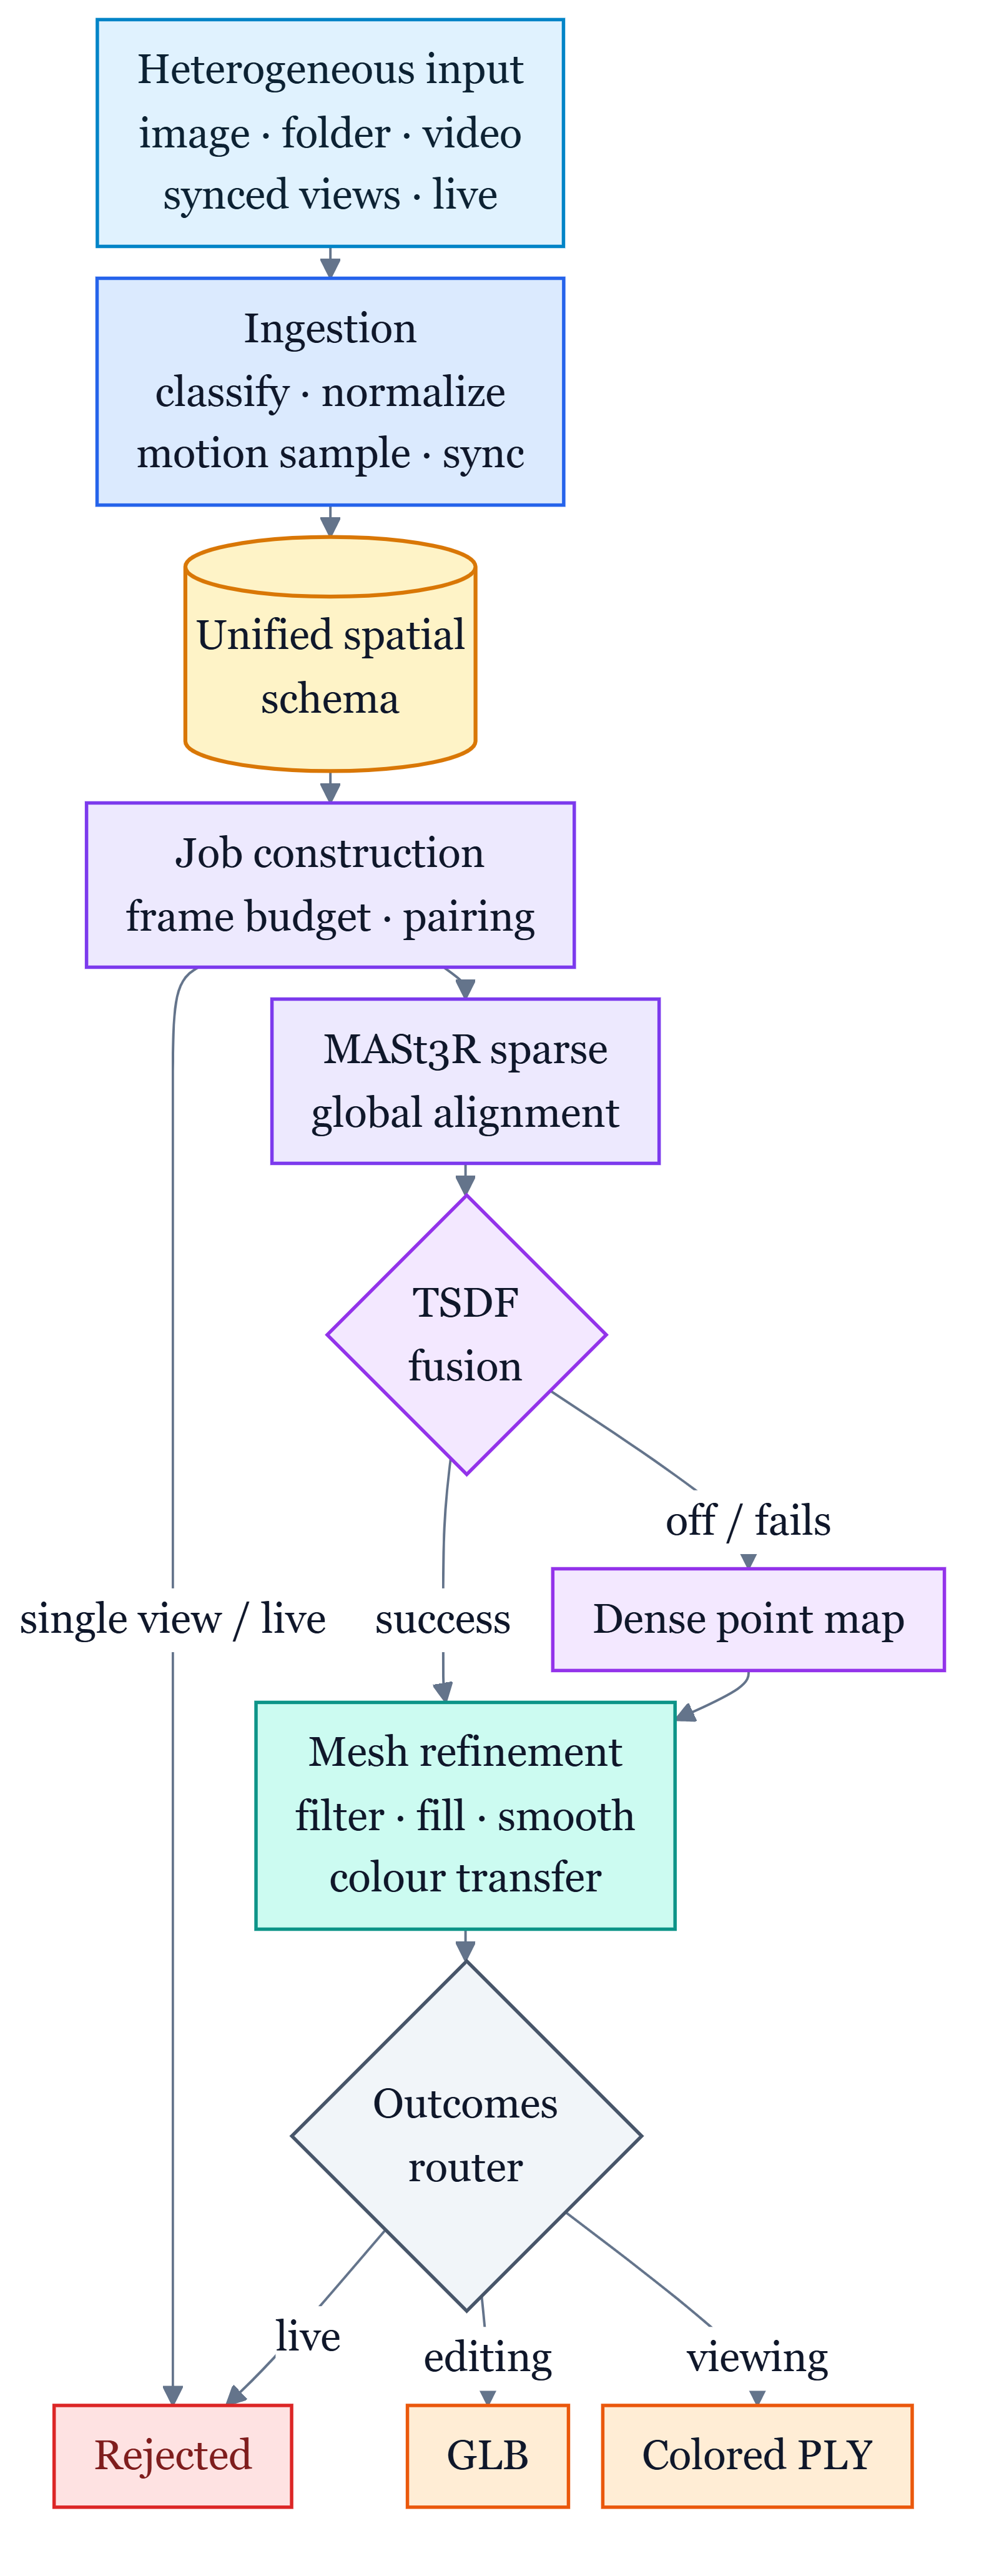
\includegraphics[width=0.6\columnwidth]{figures/fig1-overview.png}}
\caption{End-to-end pipeline: heterogeneous media are ingested, reconstructed,
refined, and routed to use-case-specific deliverables.}
\label{fig:overview}
\end{figure}

\section{System Architecture}
\label{sec:architecture}

Four modular stages make up the architecture: media ingestion, multi-view
reconstruction, mesh refinement, and outcome routing. They can communicate
only through serializable artifacts, namely a unified schema, a reconstruction
job, a mesh file, and a set of manifests. These four artifacts are the
system's interfaces. They define what one stage can assume about the previous
one, and they are where the behavior documented in Section~\ref{sec:bench-validation} originates. Fig.~\ref{fig:overview} illustrates the flow.

\subsection{Media Ingestion}

An HTTP/WebSocket gateway with pluggable authentication and rate limiting
ingests single images, image folders, videos, video folders, and live
WebSocket frames. MIME type and file extension determine which processing
track a payload enters. Mixed or unrecognized payloads are rejected outright,
never partially processed. Normalization then follows on the batch track:
images are resized while aspect ratio and EXIF metadata are preserved, and
videos are probed using FFmpeg and sampled by a motion-adaptive sampler whose
interval shortens during motion and lengthens across static spans. When the
input is a video folder, a multi-source synchronizer estimates a per-source
clock offset by matching motion signatures against the source with the most
frames, then aligns frames to that anchor by nearest timestamp. On the live
track, frames are buffered instead in a bounded ring buffer with explicit
backpressure. Oversized payloads are denied, and a full buffer evicts its
oldest frame. Compute priority goes first to live work.

\subsection{Unified Spatial Representation}

Both tracks converge into a single serializable schema, which holds source
metadata, frame references, temporal information, per-frame intrinsics, and
synchronization state. Two benefits result at this boundary between ingestion
and reconstruction. Ingestion is decoupled from reconstruction, so that each
stage encodes as little as possible about the other's internal workings. A
normalized input also becomes replayable, which lets reconstruction
experiments run against a fixed frame set instead of the original capture.

\subsection{Multi-View Reconstruction}
\label{sec:reconstruction}

An explicit reconstruction job is created during the reconstruction stage. The
mode of operation depends on the type of input used: an image folder is
processed as multi-view, a single video as a video-sequence, and a folder of
videos as synchronized-views. Since alignment requires at least two views of
one subject, single images and live streams are rejected. Because video is
redundant, a configurable frame budget applies to each job. Above that budget
the highest-motion frames are retained in preference to a uniform subsample.
When processing synchronized captures, the budget applies to entire groups
rather than to individual frames, so cross-camera groupings remain intact.
Pairing then occurs either through a complete scene graph or by sliding
window, the latter preferred for videos and larger image sets. On
synchronized-views jobs, cross-camera pairings form within each group, so that
simultaneous observations are matched directly. Frames then proceed to pairing
in motion-rank order, not capture order. Section~\ref{sec:bench-validation}
evaluates this cross-stage interaction.

Prior to alignment, the pipeline selects an execution device among CUDA, CPU,
and Metal backends, seeds the Python, NumPy, and PyTorch generators if a seed
has been supplied, and converts an EXIF 35~mm-equivalent focal length into the
per-image intrinsic matrix. MASt3R then performs sparse global alignment, with
intermediate results cached to disk so that repeated runs over the same frames
reuse prior work. TSDF fusion may optionally precede geometry export. If
fusion is disabled by user option, or fails under memory or runtime pressure,
the pipeline falls back to a dense point-map export and records the event. GLB
is the default output format for the colored mesh, with OBJ and PLY also
supported, and a confidence threshold discards low-confidence points. A
confidence-masked dense point cloud is written alongside it. Recorded in the
run manifest are the model, device, input resolution, pairing strategy,
thresholds, seed, and reproducibility metadata.

\subsection{Mesh Refinement}

So that operator and threshold settings need not be chosen per model by a
human working in an interactive tool, every mesh undergoes a single fixed
procedure during the refinement stage. Validation occurs first: container
formats such as GLB scenes are unwrapped, and meshes are rejected if they are
empty or if their vertices carry non-finite coordinates. Mode then determines
how components are processed. Under object mode, only the largest connected
component remains. Under room mode, the mesh is broken down into bodies, every
component above a minimum cell count is kept, and the survivors are merged,
preserving scenes that were legitimately created from multiple parts. Holes in
the mesh boundary are closed up to a maximum size derived from the bounding-
box diagonal. Where the geometry is thin and open along one axis, closure is
skipped, so that an intentionally planar capture is preserved.

Taubin smoothing reduces surface noise without shrinking the mesh, as
repeatedly applying Laplacian filters can do; under room mode, feature edges
above a configurable angle are additionally preserved. Finalization then
merges coincident points, triangulates, optionally decimates to a target
reduction, and recomputes outward-facing normals. Because smoothing and
decimation modify the vertex set, vertex colors are transferred to the cleaned
mesh by a nearest-point operation, which preserves appearance through the
geometric processing. The interface between these two stages must hold that
invariant, and Section~\ref{sec:bench-validation} verifies it. Open boundary
edges are counted in a final pass, which flags the mesh watertight or not and
treats a non-watertight result as a warning that does not terminate the
workflow. A refinement manifest records input and output counts, the
watertightness result, and any warnings.

\subsection{Application-Specific Deliverables}

Compatibility between source type and use case is a contract at the outcomes
stage, not a default. Each use case declares the source types it can
meaningfully consume; every other combination is rejected with a routing error
before anything is exported. All 24 combinations route or reject correctly in
our benchmark (Table~\ref{tab3}). A Blender-ready GLB leaves by the editing
pathway. The viewing pathway packages the confidence-masked point cloud into a
colored PLY, short of a full Gaussian Splatting representation. Defined at the
routing level, the live pathway rejects requests explicitly.

\section{Results and Discussion}

\subsection{Computational Performance}
\label{sec:comp-performance}

% Two log-log panels side by side (triangle-count-only panel dropped; Table I's
% removal made the caption reference this figure's own (b)-panel dashed line
% instead of a table row). Generated by trim-refine-scaling-figure.py at
% exactly \columnwidth, so no height cap is needed and the point sizes set in
% that script are the ones that reach the page.
\begin{figure}[tbp]
\centerline{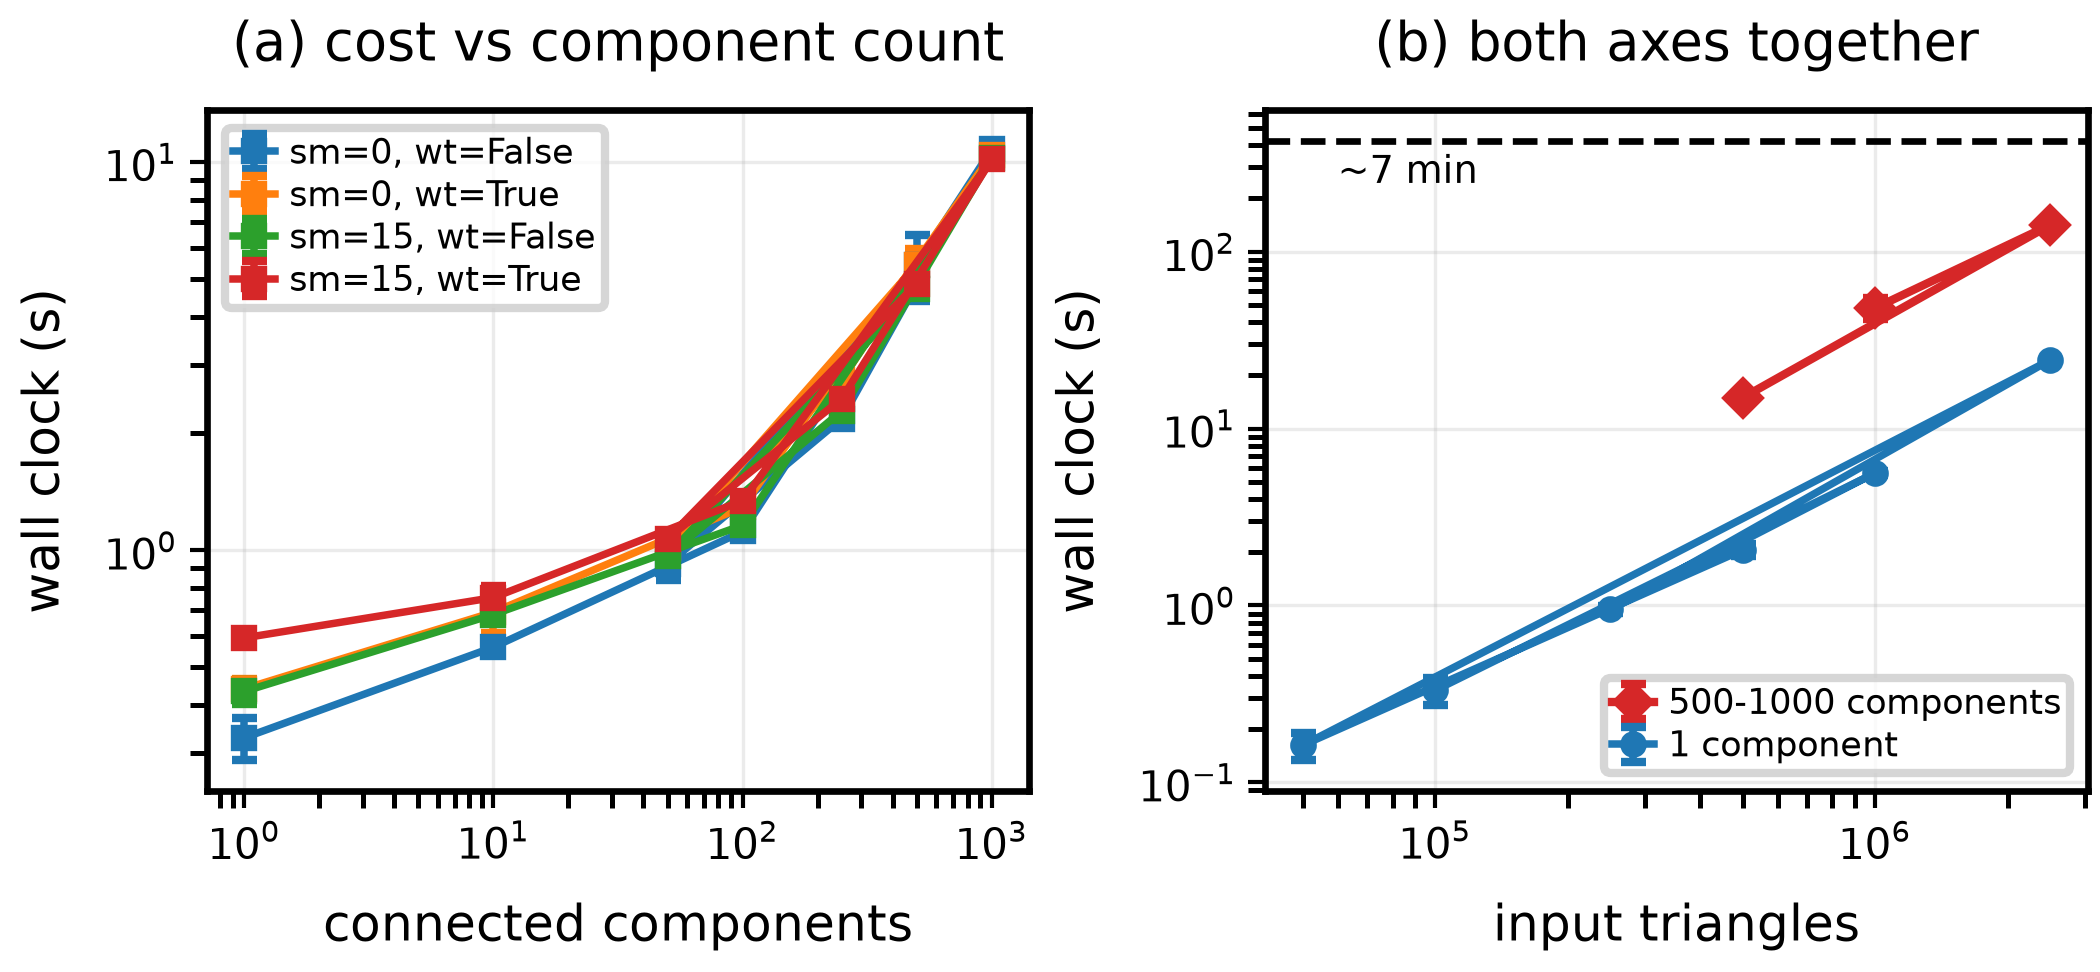
\includegraphics[width=\columnwidth]{figures/fig9-refine-scaling.png}}
\caption{Refinement wall time vs.\ (a) component count and (b) component and
triangle count together, log-log, error bars SD over 3 repeats. Dashed line
in (b) marks the $\sim$7-minute combined-load case.}
\label{fig:refine-scaling}
\end{figure}

Per-component processing overhead dominates refinement cost in the current
implementation; triangle count matters less. Taken alone on a single connected
mesh, triangle count is only mildly super-linear: a log-log fit over 50K--2.5M
triangles yields an exponent of 1.16--1.31 across the eight
configuration/geometry combinations, with $R^2 > 0.98$ throughout, and the
default configuration adds no more than 23\% over the smoothing-off baseline.
The stronger driver is component count. At a fixed $\sim$96,000 triangles
(Fig.~\ref{fig:refine-scaling}(a)), cost grows 23x between 1 and 1,000
components on the pooled means, and 17--33x across the four configurations.

Nor is that growth a clean power law; the endpoint ratio alone would overstate
how evenly it accumulates. Fitted over the whole component ladder, a single
log-log exponent of 0.39--0.48 (0.43 pooled) fits poorly, at $R^2 = 0.85$,
because the curve has a knee. Its local exponent is 0.22 from 1 to 100
components and 0.94 from 100 to 1,000. Below roughly 100 components,
fragmentation is nearly free: 0.45~s to 1.23~s, under 3x over two decades.
Above that point cost rises close to linearly in component count, supplying
the remaining $\sim$8.5x. Fragmentation thus behaves as a threshold rather
than a gradient. Refinement stays cheap until component count reaches the low
hundreds, past which each additional component costs roughly a fixed amount.
The two axes are also super-additive: the combined configuration costs roughly
4x the additive prediction and reaches the $\sim$7-minute regime marked in
Fig.~\ref{fig:refine-scaling}(b).

\begin{table}[tbp]
\caption{Mean Refinement Cost over 5 Runs}
\begin{center}
\footnotesize
\begin{tabular}{|p{2.1cm}|p{2.05cm}|p{2.05cm}|}
\hline
\textbf{Stage} & \textbf{Large Mesh} & \textbf{Fragmented Mesh} \\
\hline
Component filtering & 0.90 s (12.0\%) & 9.64 s (95.9\%) \\
\hline
Hole filling & 0.45 s (6.0\%) & 0.03 s (0.3\%) \\
\hline
Smoothing & 0.96 s (12.7\%) & 0.13 s (1.3\%) \\
\hline
Finalization & 4.06 s (53.7\%) & 0.16 s (1.6\%) \\
\hline
Watertightness check & 1.19 s (15.7\%) & 0.10 s (0.9\%) \\
\hline
\textbf{Total} & \textbf{7.55 s} & \textbf{10.06 s} \\
\hline
\end{tabular}
\label{tab-stage-profile}
\end{center}
\end{table}

Table~\ref{tab-stage-profile} attributes this cost to different substeps in
each regime. Finalization dominates on a large connected mesh, at 53.7\%,
mostly point deduplication and normal recomputation. On a many-component mesh,
component filtering dominates instead, at 95.9\%, driven by repeated per-piece
processing during body splitting. A mechanical explanation for the knee
follows. Body splitting runs each connected component through a separate
processing pass, so once component count grows large enough for that loop to
dominate the fixed per-mesh work, cost tracks component count directly. The
obvious optimization is a batched connected-component labeling pass, which we
did not implement for this study.

This cost belongs to an interface, not to a stage. What sets refinement's
runtime is a structural property of the mesh that the reconstruction stage
happens to hand it, and no benchmark of refinement on a single connected mesh
would reveal it. TSDF fusion can become expensive in a similar way; its
fallback to dense point-map export degrades gracefully, at the price of an
output representation that depends on available resources.

\subsection{Determinism and Repeat-Run Behavior}

Run manifests record the reconstruction model, device, pairing strategy, seed,
and configuration, which supports repeatable re-execution on the same
hardware. On three scenes (\texttt{scan24}, \texttt{scan37}, \texttt{scan40}),
a small GPU benchmark tested this, running each twice on one Tesla~T4 under
one seed with the cache cleared between runs. Hausdorff-95 and Chamfer
distance between repeats were exactly 0.0, point counts matched, and exported
GLB files were byte-identical by SHA-256; this held regardless of PyTorch's
deterministic-algorithms mode, which added $\sim$21\% wall time without
measurably improving repeatability here. Reproducibility in the general sense
is not established by six runs on one device. What they show is narrower: that
the manifest captures enough state to reproduce a run bit-for-bit when
hardware is held fixed, and that the deterministic-kernel setting is not what
buys it.

\subsection{Component and Integration Correctness}
\label{sec:bench-validation}

Controlled validation of the individual components and their interfaces is
summarized in Table~\ref{tab3}, where every number traces to a committed CSV.
These are contract checks on a synthetic, single-body protocol. Component
filtering removes every injected fragment, and object and room mode converge
to the same output, as they should on a single body and would not on real
multi-body scenes. As injected corruption is removed, distance to the clean
ground truth improves monotonically (Fig.~\ref{fig:refine-quality}(a)--(b)),
which the injection protocol guarantees by construction. The informative
comparison there is between smoothing operators: Taubin holds mesh volume
within 0.15\% of the unsmoothed baseline, against 0.52\% drift for Laplacian
(Fig.~\ref{fig:refine-quality}(c)). Synchronization, motion-sampling, routing,
and color-transfer correctness are established by the remaining rows.

\textbf{Frame ordering and pairing locality.} Motion-ranked retention above the
frame budget (Section~\ref{sec:reconstruction}) changes frame ordering before
sliding-window pairing, which assumes capture order. Re-sorting the retained
frames into capture order reduces the median pair-index gap from 184.5 to 27.8
across the three over-budget schedules. That is 6.6x pooled and 4.4x to 10x
per schedule, at no additional cost, and complete pairing is unaffected
because it does not depend on order. On its own neither stage is incorrect:
selection returns the frames it was asked for, and pairing windows the
sequence it is given. Only when the two are put together does the defect
appear, and no test that exercises either stage alone would find it. Its
effect on reconstruction quality we do not measure.

Together these establish component-level correctness against synthetic ground
truth, integration correctness across the routing, manifest, and color-transfer
invariants, and systems-level behavior under controlled conditions, covering
scaling, determinism, and robustness to injected corruption. End-to-end
reconstruction accuracy against captured ground truth is a separate question,
which the protocols in Section~\ref{sec:future-work} address.

% 2x2: panels (a)-(c) plus the legend (a) and (b) share in the fourth cell.
% Generated by trim-refine-quality-figure.py at exactly \columnwidth. It was
% three stacked panels behind a height=0.62\textheight cap, which printed
% ~5.7 in -- over half a column for three small line plots.
\begin{figure}[tbp]
\centerline{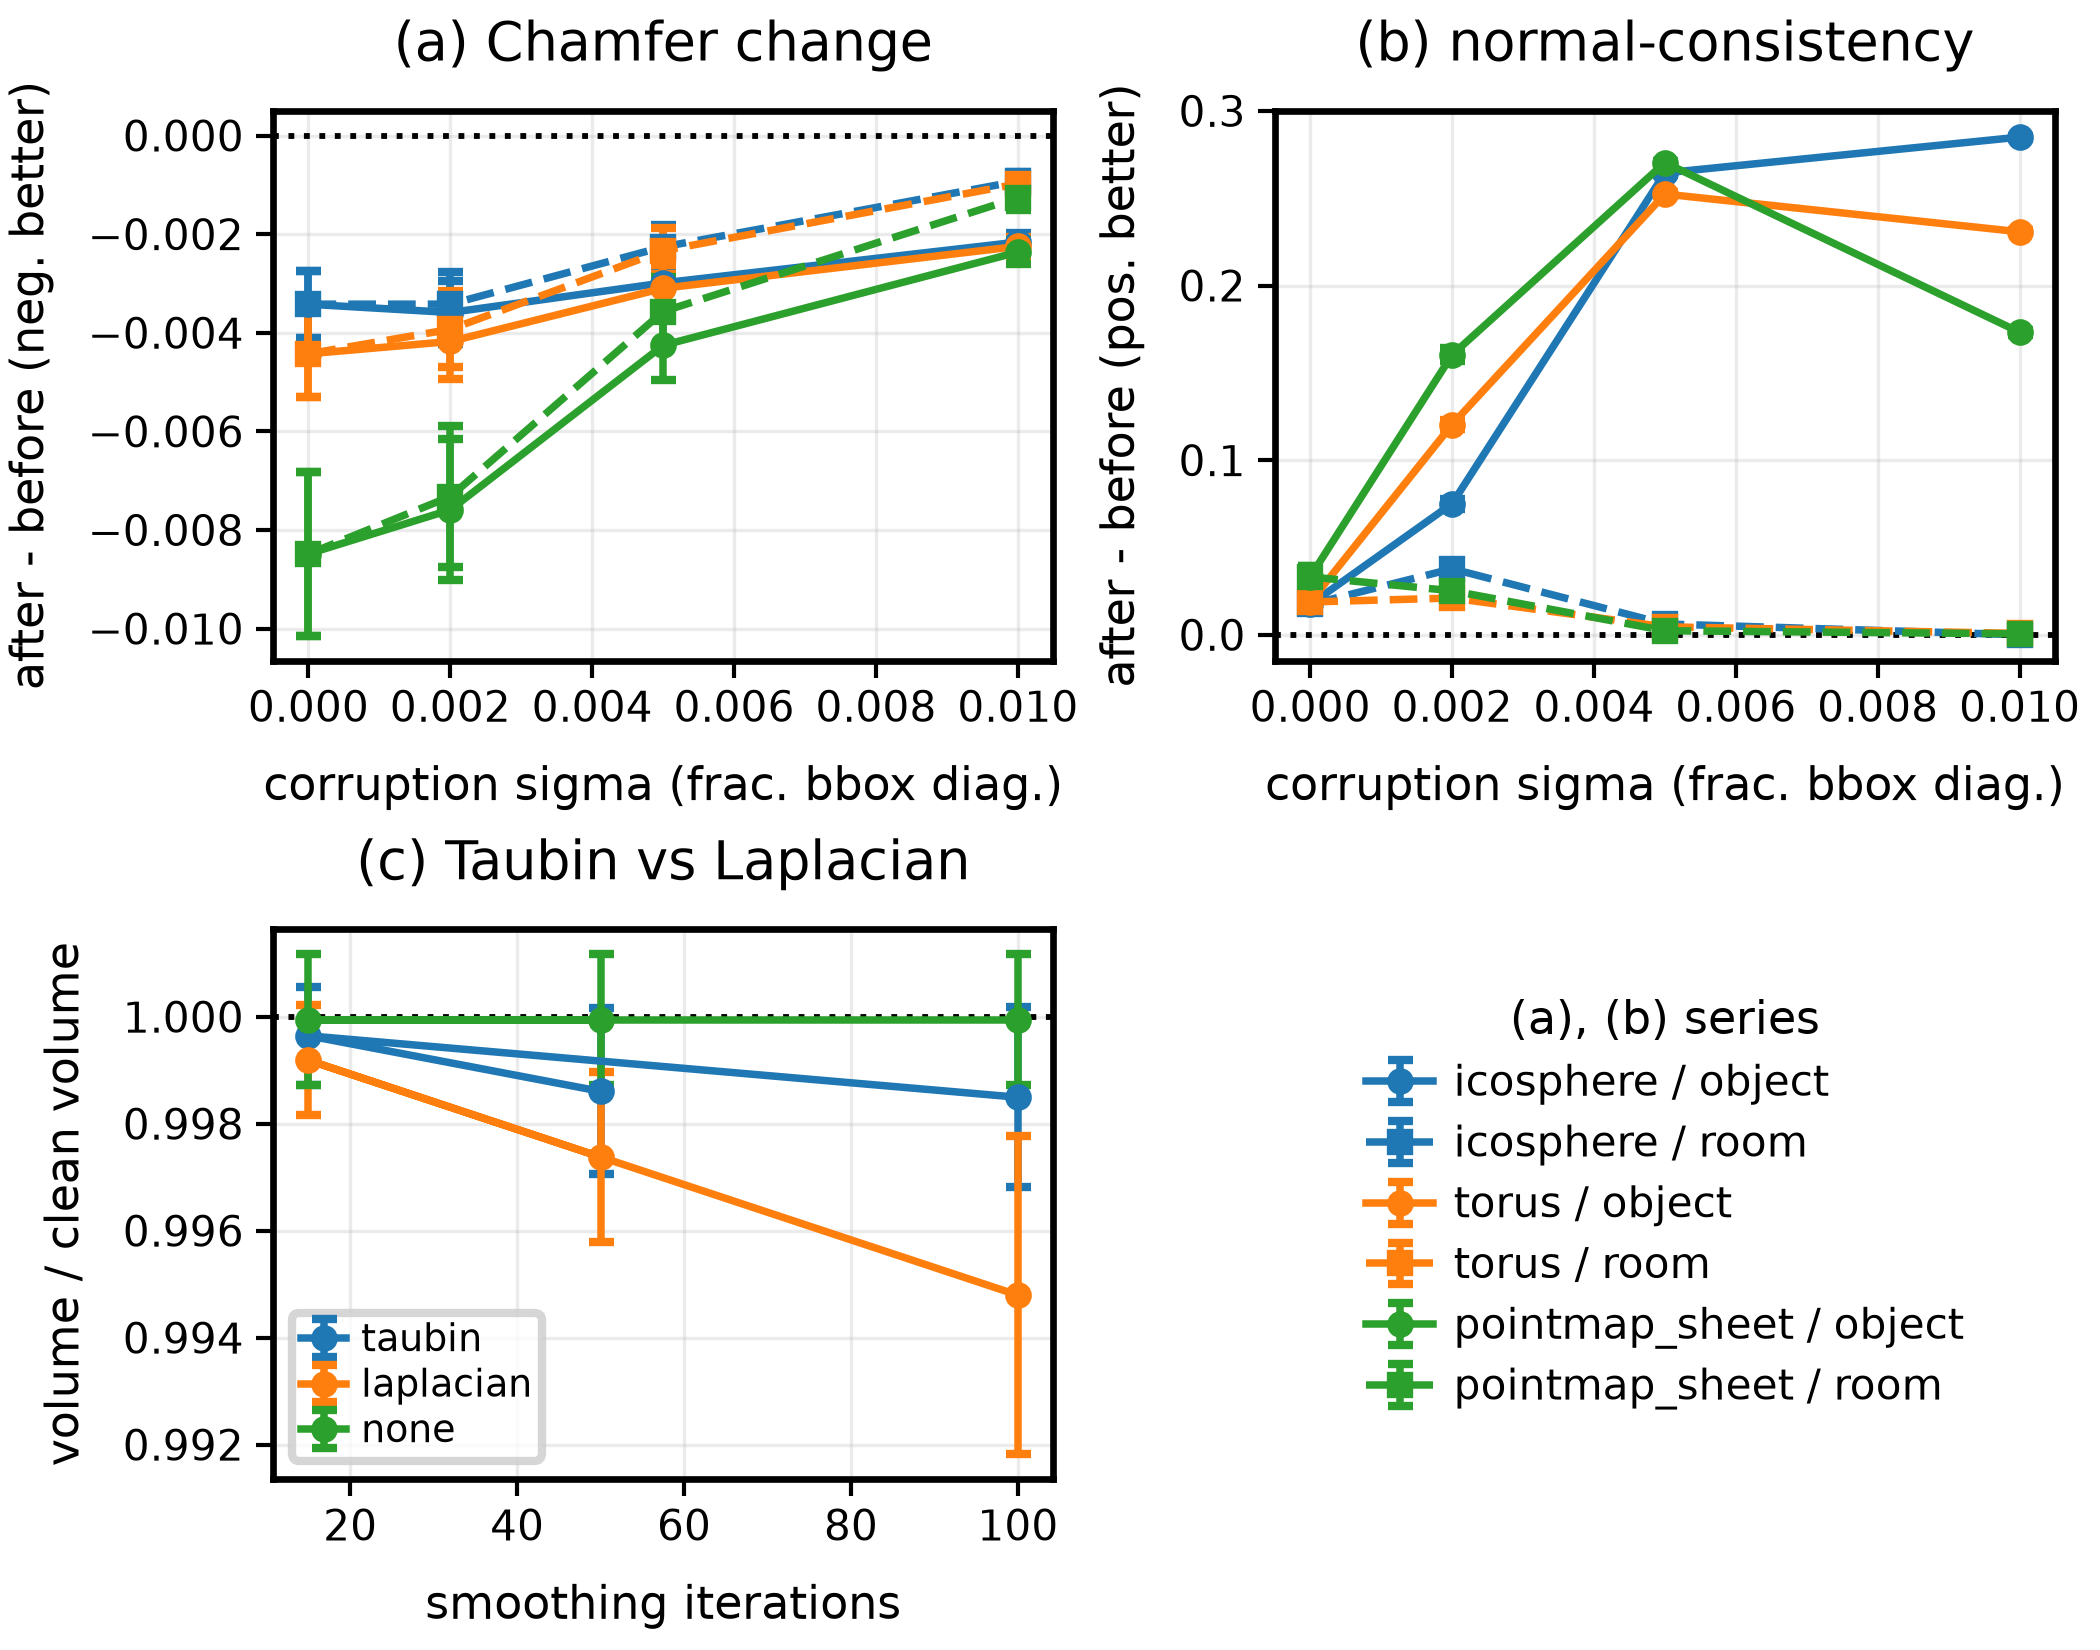
\includegraphics[width=\columnwidth]{figures/fig12-refine-quality.png}}
\caption{Refinement effect vs.\ corruption level: (a) Chamfer distance,
(b) normal consistency, and (c) volume retained under Taubin vs.\ Laplacian
smoothing. Error bars are SEM over holes, fragments, and seeds.}
\label{fig:refine-quality}
\end{figure}

\begin{table}[tbp]
\caption{Component and Integration Correctness Checks (CPU-Only, Synthetic Conditions)}
\begin{center}
\footnotesize
\begin{tabular}{|>{\raggedright\arraybackslash}p{1.7cm}|>{\raggedright\arraybackslash}p{2.0cm}|>{\raggedright\arraybackslash}p{3.7cm}|}
\hline
\textbf{Component} & \textbf{Evaluation} & \textbf{Key Result} \\
\hline
Component filtering & 0/5/20 injected fragments & All injected fragments removed; object and room mode converge, as expected on a single body \\
\hline
Frame selection / pairing & 3 over-budget video schedules & Re-sorting before pairing reduces median pair-index gap 184.5 $\to$ 27.8 (6.6x pooled, 4.4--10x per schedule) \\
\hline
Synchronization & 4,455 trials, 0--640~ms offset, jitter, 2--4 sources & 2.14~ms mean absolute offset error; 100\% sign accuracy; 99.8\% group formation \\
\hline
Motion sampling & Controlled motion windows & 1.2--2.5x concentration over uniform sampling; collapses toward 1.0x for low-magnitude motion \\
\hline
Routing & 24 source-type / use-case combinations & 100\% correct routing or rejection, no default fallthrough \\
\hline
Color transfer & Analytic color field & $<$1/255 mean per-channel error across all settings \\
\hline
\end{tabular}
\label{tab3}
\end{center}
\end{table}

\subsection{Illustrative End-to-End Trace}

The results above are the paper's evidence. This subsection adds a single traced
run ($n=1$) of the offline workflow of Fig.~\ref{fig:overview} on a real
eight-view CO3D \emph{teddybear} capture. We include it to show the assembled
pipeline running end to end at full scale, and to check whether the cost model of
Section~\ref{sec:comp-performance} predicts where the time goes. One run
supports neither a timing claim nor a quality claim. Table~\ref{tab2} reports
the per-stage timings for that purpose only.

\begin{table}[tbp]
\caption{Stage Timings for CO3D Teddybear Multi-View Capture}
\begin{center}
\footnotesize
\begin{tabular}{|p{2.4cm}|p{2.0cm}|p{1.4cm}|}
\hline
\textbf{Stage} & \textbf{Output} & \textbf{Time} \\
\hline
Sparse alignment (MASt3R) & 56 pairs & 1533.2 s \\
\hline
Mesh export & 1.90M tri / 669K pts, 64.3\% conf. retained & 71.8 s \\
\hline
\textit{Reconstruction total} & & \textit{1605.0 s} \\
\hline
Component filtering & 1.90M $\to$ 0.41M cells & 3069.3 s \\
\hline
Hole filling & & 0.33 s \\
\hline
Taubin smoothing & & 0.12 s \\
\hline
Finalization & & 0.85 s \\
\hline
Vertex-color transfer & & 0.18 s \\
\hline
Watertightness check & non-watertight & 0.53 s \\
\hline
\textit{Refinement total} & 412K cells / 112K pts & \textit{3071.3 s} \\
\hline
\textbf{Reconstruction + refinement} & & \textbf{4676.3 s ($\approx$78 min)} \\
\hline
\end{tabular}
\label{tab2}
\end{center}
\end{table}

Alignment peaked at 5259.6 MB resident and retained 64.3\% of points after
confidence masking. Total runtime was $\approx$78 min. Component filtering alone
accounted for 99.9\% of refinement wall time, and every other substep together
cost under one second (Table~\ref{tab2}). This is the fragmentation regime of
Section~\ref{sec:comp-performance} at full scale. The mesh has 1.90M triangles
and sits far past the component-count knee, where the benchmark predicts
component filtering will swamp everything else. It does. The output was
correctly flagged as non-watertight and the warning did not halt the workflow,
so the pipeline reports geometry defects instead of terminating on them.

% Composed side by side by compose-case-study-figure.py at exactly
% \columnwidth, so no height cap is needed: the file's own aspect ratio prints
% it ~1.2 in tall. It was previously two stacked panels behind a
% height=0.44\textheight cap, which cost ~4 in of column for two photographs.
\begin{figure}[tbp]
\centerline{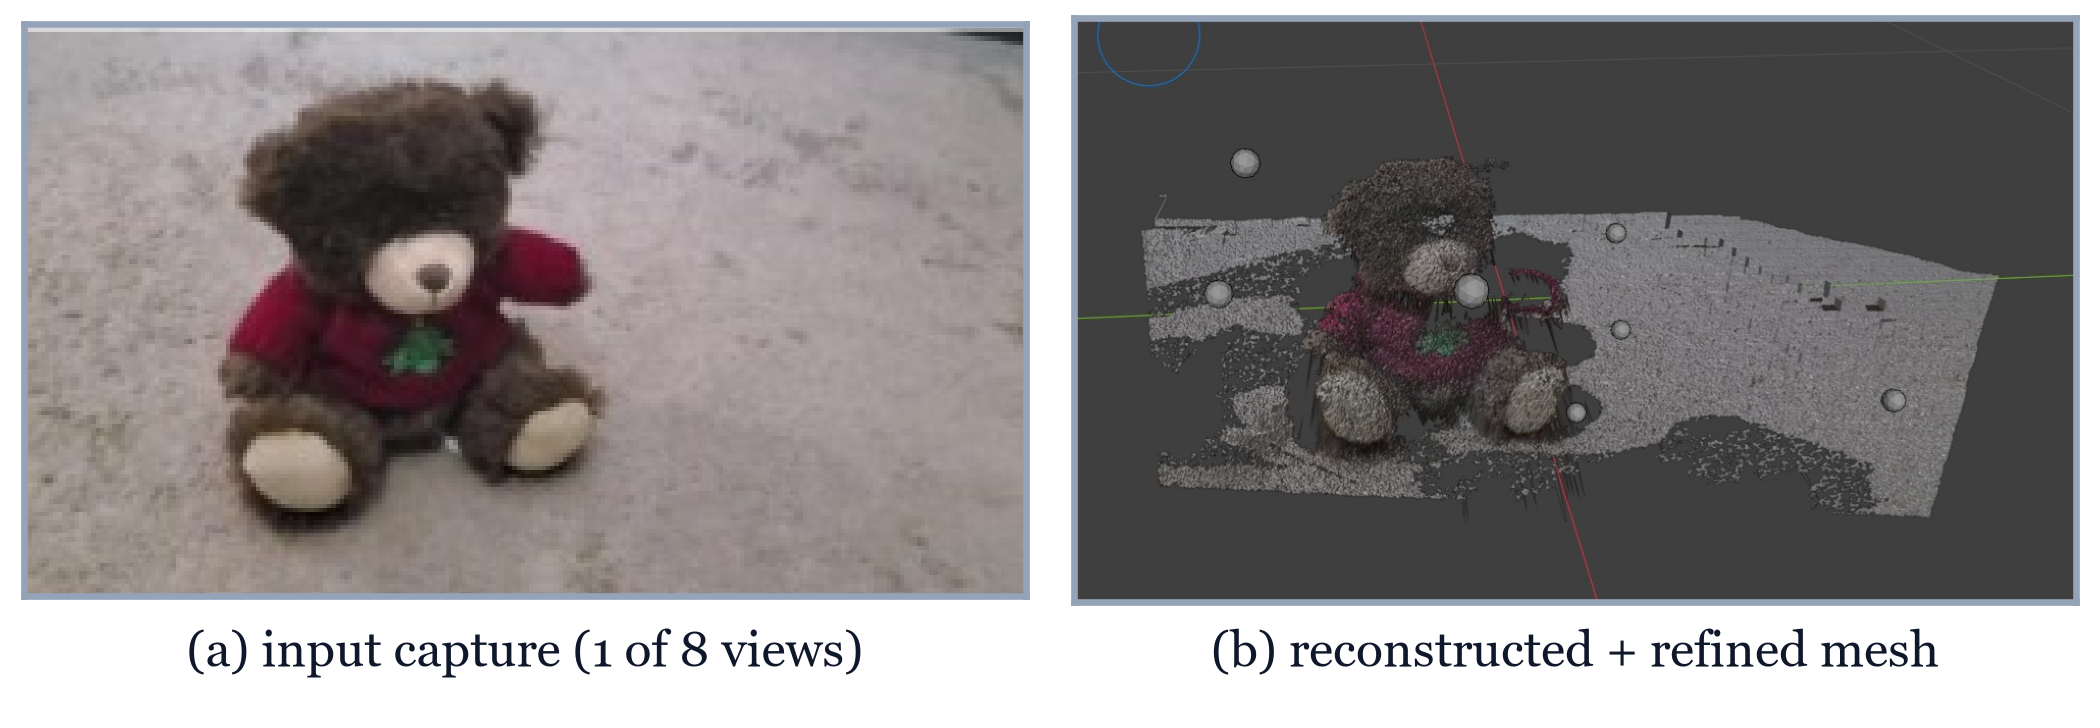
\includegraphics[width=\columnwidth]{figures/fig6-case-study-validation.png}}
\caption{Case-study result: (a) input photograph and (b) reconstructed,
refined mesh. The subject is recognizable, with residual background
fragments and surface holes visible.}
\label{fig:validation}
\end{figure}

Fig.~\ref{fig:validation} shows the result qualitatively: the subject is
recognizable and the defects of raw reconstruction are visibly corrected, though
residual background geometry remains. No quantitative reconstruction accuracy is
claimed from it.

\section{Conclusions}

z-shift is a systems architecture of independently replaceable stages
communicating through explicit artifacts (Fig.~\ref{fig:overview}), and not a
new reconstruction network. Its findings concern how those stages fit
together. Correct at the selection stage, frame ordering nonetheless breaks
pairing locality at the next one, and restoring capture order recovers a 6.6x
pair-index gap for free. Mesh fragmentation, a structural property of what
reconstruction hands refinement, governs refinement cost in this
implementation far more than triangle count does, and it does so as a
threshold rather than a gradient: cost is nearly flat below roughly 100
components, then close to linear in component count, reaching 23x at 1,000.
That shape, more than the endpoint ratio, is what makes cost predictable in
advance, since a single structural property of the incoming mesh determines
which regime a run lands in. Repeat runs of a fixed configuration on one GPU
were deterministic down to the byte, with identical SHA-256 mesh hashes. None
of this would surface from a benchmark of a single stage on its own. Component
correctness does not imply system correctness or predictable system cost.
Outside this evaluation there remains end-to-end reconstruction accuracy
against captured ground truth (Section~\ref{sec:future-work}).

\section{Limitations and Future Work}
\label{sec:future-work}

Three principal limitations attach to the prototype. Real-time delivery is
incomplete: WebSocket ingestion works, but RTSP/WebRTC and the live outcome
route are unimplemented, and viewing exports a colored point cloud instead of
Gaussian Splatting. Refinement is CPU-bound and expensive on fragmented
meshes. There is no end-to-end ground-truth reconstruction benchmark.
Reconstruction requires at least two views, and authentication, rate limiting,
and streaming state remain in-memory and single-process, reflecting research-
prototype status.

Component-, integration-, and systems-level behavior is therefore what our
evaluation establishes, not reconstruction accuracy. Quantitative comparison
against classical MVS, DUSt3R, and MASt3R baselines, using Chamfer distance,
point-to-surface error, and F-score, is the priority for future work.

\begin{thebibliography}{00}
\bibitem{b1} R. Hartley and A. Zisserman, Multiple View Geometry in Computer Vision, 2nd ed. Cambridge, U.K.: Cambridge Univ. Press, 2004.
\bibitem{b2} J. L. Sch\"onberger and J.-M. Frahm, ``Structure-from-motion revisited,'' in Proc. IEEE CVPR, 2016, pp. 4104--4113.
\bibitem{b3} S. M. Seitz, B. Curless, J. Diebel, D. Scharstein, and R. Szeliski, ``A comparison and evaluation of multi-view stereo reconstruction algorithms,'' in Proc. IEEE CVPR, 2006, pp. 519--528.
\bibitem{b4} Y. Furukawa and C. Hern\'andez, ``Multi-view stereo: A tutorial,'' Foundations and Trends in Computer Graphics and Vision, vol. 9, no. 1--2, pp. 1--148, 2015.
\bibitem{b6} B. Mildenhall, P. P. Srinivasan, M. Tancik, J. T. Barron, R. Ramamoorthi, and R. Ng, ``NeRF: Representing scenes as neural radiance fields for view synthesis,'' in Proc. ECCV, 2020, pp. 405--421.
\bibitem{b7} T. M\"uller, A. Evans, C. Schied, and A. Keller, ``Instant neural graphics primitives with a multiresolution hash encoding,'' ACM Trans. Graph., vol. 41, no. 4, 2022.
\bibitem{b8} B. Kerbl, G. Kopanas, T. Leimk\"uhler, and G. Drettakis, ``3D Gaussian splatting for real-time radiance field rendering,'' ACM Trans. Graph., vol. 42, no. 4, 2023.
\bibitem{b9} J. T. Barron et al., ``Mip-NeRF 360: Unbounded anti-aliased neural radiance fields,'' in Proc. IEEE/CVF CVPR, 2022, pp. 5470--5479.
\bibitem{b10} A. Chen et al., ``MVSNeRF: Fast generalizable radiance field reconstruction from multi-view stereo,'' in Proc. IEEE/CVF ICCV, 2021, pp. 14124--14133.
\bibitem{b11} A. Yu et al., ``pixelNeRF: Neural radiance fields from one or few images,'' in Proc. IEEE/CVF CVPR, 2021, pp. 4578--4587.
\bibitem{b14} S. Wang, V. Leroy, Y. Cabon, B. Chidlovskii, and J. Revaud, ``DUSt3R: Geometric 3D vision made easy,'' in Proc. IEEE/CVF CVPR, 2024.
\bibitem{b15} V. Leroy, Y. Cabon, and J. Revaud, ``Grounding image matching in 3D with MASt3R,'' in Proc. IEEE/CVF ECCV, 2024.
\bibitem{b16} G. Taubin, ``A signal processing approach to fair surface design,'' in Proc. ACM SIGGRAPH, 1995, pp. 351--358.
\bibitem{b17} M. Garland and P. S. Heckbert, ``Surface simplification using quadric error metrics,'' in Proc. ACM SIGGRAPH, 1997, pp. 209--216.
\bibitem{b18} P. Cignoni, M. Callieri, M. Corsini, M. Dellepiane, F. Ganovelli, and G. Ranzuglia, ``MeshLab: An open-source mesh processing tool,'' in Proc. Eurographics Italian Chapter Conference, 2008, pp. 129--136.
\bibitem{b19} M. Botsch et al., Polygon Mesh Processing. Natick, MA, USA: A K Peters/CRC Press, 2010.
\bibitem{b21} B. Curless and M. Levoy, ``A volumetric method for building complex models from range images,'' in Proc. ACM SIGGRAPH, 1996, pp. 303--312.
\bibitem{b22} R. A. Newcombe et al., ``KinectFusion: Real-time dense surface mapping and tracking,'' in Proc. IEEE ISMAR, 2011, pp. 127--136.
\bibitem{b23} M. Kazhdan, M. Bolitho, and H. Hoppe, ``Poisson surface reconstruction,'' in Proc. Eurographics Symposium on Geometry Processing, 2006, pp. 61--70.
\bibitem{b25} J. L. Sch\"onberger, E. Zheng, M. Pollefeys, and J.-M. Frahm, ``Pixelwise view selection for unstructured multi-view stereo,'' in Proc. ECCV, 2016, pp. 501--518.
\bibitem{b26} C. Griwodz et al., ``AliceVision and Meshroom: An open-source photogrammetric pipeline,'' in Proc. ACM Multimedia Systems Conference (MMSys), 2021, pp. 241--247.
\bibitem{b27} M. Tancik et al., ``Nerfstudio: A modular framework for neural radiance field development,'' in Proc. ACM SIGGRAPH Conference, 2023.
\bibitem{b28} Q.-Y. Zhou, J. Park, and V. Koltun, ``Open3D: A modern library for 3D data processing,'' arXiv:1801.09847, 2018.
\bibitem{b29} K. M. Jatavallabhula et al., ``Kaolin: A PyTorch library for accelerating 3D deep learning research,'' arXiv:1911.05063, 2019.
\bibitem{b34} A. Dai et al., ``ScanNet: Richly-annotated 3D reconstructions of indoor scenes,'' in Proc. IEEE CVPR, 2017, pp. 5828--5839.
\end{thebibliography}

\end{document}